
%(BEGIN_QUESTION)
% Copyright 2007, Tony R. Kuphaldt, released under the Creative Commons Attribution License (v 1.0)
% This means you may do almost anything with this work of mine, so long as you give me proper credit

Processes are sometimes classified according to the types of electrical component that behave similarly: {\it resistive} or {\it capacitive}.  What exactly is a ``resistive'' process (sometimes called a {\it self-regulating} process), and a ``capacitive'' process (sometimes called an {\it integrating} or {\it ramping} process)?  Give one example of each type of process.

\underbar{file i01676}
%(END_QUESTION)





%(BEGIN_ANSWER)

A {\it resistive} (``self-regulating'') process is one where changes in the manipulated variable result in proportional changes to the process variable.  In other words, if the manipulated variable ``steps'' by a certain amount, the process variable will also ``step'' by a certain amount (although this ``step'' response may not necessarily be immediate).

An example of a resistive process is a liquid flow control system.  Step-changes in valve position result in proportional step-changes to the flow rate.
 
Resistive processes are inherently stable.  So long as the manipulated variable and ``load(s)'' on the process remain steady, the process variable will naturally stabilize at some point.
 
Consider the response of a resistor to a changing current through it:

$$\includegraphics[width=15.5cm]{i01676x01.eps}$$

\vskip 10pt

\filbreak

A {\it capacitive} (``integrating'') process is one where changes in the manipulated variable result in proportional changes to the process variable's {\it rate-of-change} over time.  In other words, if the manipulated variable ``steps'' by a certain amount, the process variable will alter its rate-of-change over time.

An example of a capacitive process is a liquid level control system.  Step-changes in valve position result in changes to the {\it rate} of level change over time.

Capacitive processes are inherently {\it un}stable.  The process variable will stabilize if and only if the manipulated variable precisely matches the process load(s), since the process variable is a function of the integral of the difference between process input and process output.

It should be noted that most real processes exhibit a combination of ``resistive'' and ``capacitive'' tendencies, but that often one of these characteristics predominates over the other.

Consider the response of a capacitor to a changing current through it:

$$\includegraphics[width=15.5cm]{i01676x02.eps}$$


%(END_ANSWER)





%(BEGIN_NOTES)


%INDEX% Control, process characteristics: self-regulating versus integrating

%(END_NOTES)


